\section{子群、陪集与群作用}
\label{sec:04-Discrete-Mathematics/06-Groups-and-Symmetry/02}

把上一节那张正方形卡片按住一个角，不许它离开桌面上的那个位置，其余动作随便做。还剩几种？两种：什么都不做，以及沿这个角所在的对角线翻折。八个动作里，只有这两个对该角网开一面。

换个按法，按住卡片的中心不放而只禁止翻面，剩下的是四个旋转。同样是从八个里挑出一部分，挑出来的那部分自己仍然能首尾相接：两个旋转连着做还是旋转，撤销一个旋转还是旋转。

于是群的内部并不均匀，里面嵌着能够独立运转的小系统。这一节顺着三个递进的问题走：哪些子集自己就能构成群（子群）？用一个子群当尺子去量整个群，会量出什么（陪集与 Lagrange 定理）？把群搭到一个外部集合上之后，怎样说清``这两个对象只差一个对称''（群作用与轨道）？

\subsection{子群：一条判据打包四条公理}

群 \(G\) 的非空子集 \(H\) 称为子群，若 \(H\) 在 \(G\) 的运算下自己也是群，记作 \(H\le G\)。逐条核验四条公理是浪费——结合律从 \(G\) 白拿，剩下三条可以用一句话打包：对任意 \(a,b\in H\)，都有

\[
ab^{-1}\in H.
\]

取 \(a=b\) 得 \(e\in H\)；再取 \(a=e\) 得 \(b^{-1}\in H\)；有了逆元，把 \(b\) 换成 \(b^{-1}\) 就得 \(ab\in H\)。一条判据穿起三件事。

在 \(D_4\) 里试几次。\(\set{e,r,r^2,r^3}\) 过关；\(\set{e,r^2}\) 过关；\(\set{e,s}\) 过关。但 \(\set{e,r,s}\) 不行，\(rs\) 既不是这里的旋转也不是这里的翻折，跑出去了。给定任意一组元素 \(S\)，把它们连同各自的逆元用一切有限乘积组装起来，得到包含 \(S\) 的最小子群 \(\langle S\rangle\)。在 \(D_4\) 中 \(\langle r\rangle\) 是四个旋转，\(\langle s\rangle=\set{e,s}\)，而 \(\langle r,s\rangle\) 已经是整个 \(D_4\)——一个旋转加一个翻折就够生成全部对称。

\subsection{陪集把群切成等大的块}

有了子群 \(H\)，固定一个 \(g\in G\)，把 \(H\) 整体左乘 \(g\)：

\[
gH=\set{gh:h\in H}.
\]

这是左陪集。它一般不是子群——除非 \(g\in H\)，否则单位元根本不在里面。它更像 \(H\) 被平移之后的一块拓片：映射 \(h\mapsto gh\) 是 \(H\) 到 \(gH\) 的双射（逆映射是左乘 \(g^{-1}\)），所以每个陪集的元素个数都等于 \(\abs{H}\)。

陪集之间只有两种关系：完全重合，或者毫无交集。若 \(g_1H\) 与 \(g_2H\) 共用一个元素，即 \(g_1h_1=g_2h_2\)，则 \(g_2^{-1}g_1=h_2h_1^{-1}\in H\)，顺着推下去两个陪集逐元素相等。既然每个 \(g\) 至少落在自己的陪集 \(gH\) 里，这些互不相交的等大块就把 \(G\) 铺满了。

\begin{center}
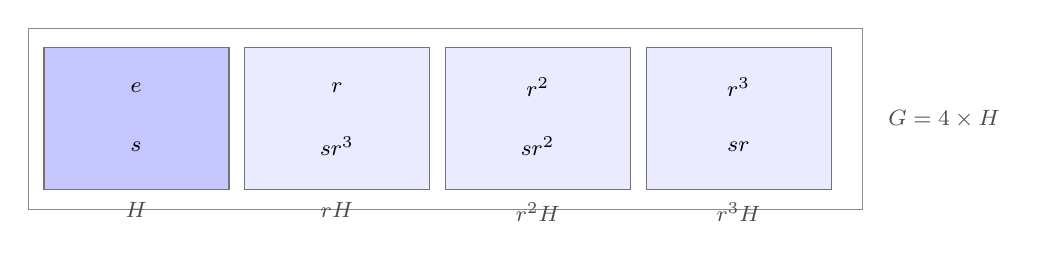
\begin{tikzpicture}[x=1cm,y=1cm,font=\footnotesize]
  \draw[black!45] (-0.2,-0.55) rectangle (10.4,1.75);
  \foreach \px/\ttl/\ua/\ub/\fc in {%
    0/{H}/{e}/{s}/{blue!22},
    2.55/{rH}/{r}/{sr^3}/{blue!8},
    5.1/{r^2H}/{r^2}/{sr^2}/{blue!8},
    7.65/{r^3H}/{r^3}/{sr}/{blue!8}}
  {
    \begin{scope}[shift={(\px,0)}]
      \draw[black!55,fill=\fc] (0,-0.3) rectangle (2.35,1.5);
      \node at (1.17,1.0) {\(\ua\)};
      \node at (1.17,0.25) {\(\ub\)};
      \node[below,black!70] at (1.17,-0.34) {\(\ttl\)};
    \end{scope}
  }
  \node[right,black!70] at (10.6,0.6) {\(\abs{G}=4\times\abs{H}\)};
\end{tikzpicture}

\emph{取 \(H=\set{e,s}\)，四个左陪集把 \(D_4\) 的八个元素分成四块，每块两个，互不重叠。深色那块是 \(H\) 自己，其余三块是它的平移拷贝——形状相同，只是不含单位元。}
\end{center}

图上的等式就是 Lagrange 定理的全部内容。

\begin{theorem}[Lagrange]
设 \(G\) 是有限群，\(H\le G\)。则 \(\abs{H}\) 整除 \(\abs{G}\)，且商 \([G:H]=\abs{G}/\abs{H}\) 等于左陪集的个数。
\end{theorem}

证明骨架只有三句：每个陪集与 \(H\) 等势；不同陪集互不相交；所有陪集并起来是 \(G\)。三句各自都是上面推过的一行。条件对账也简单：有限性只用来保证``块数''是个数，无限群里陪集分解照样成立，只是不能写成整除关系。

把 \(H\) 取成单个元素生成的循环子群 \(\langle g\rangle\)，立刻得到：任意元素的阶整除群的阶，于是对有限群中任意 \(g\) 有 \(g^{\abs{G}}=e\)。\hyperref[sec:04-Discrete-Mathematics/04-Number-Theory/03]{``Fermat 与 Euler 定理''}正是这句话在模 \(n\) 可逆余数类乘法群上的实例：那个群的大小是 \(\varphi(n)\)，所以 \(a^{\varphi(n)}\equiv1\pmod n\)。认出一个运算构成有限群，这类结论就是免费的。

Lagrange 定理只能正着用。\(d\) 不整除 \(\abs{G}\) 时确实没有 \(d\) 阶子群；但 \(d\mid\abs{G}\) 并不保证 \(d\) 阶子群存在——12 阶的偶置换群 \(A_4\) 没有 6 阶子群，尽管 \(6\mid12\)。更不能因为某个子集的大小恰好是 \(\abs{G}\) 的因子就断定它是子群，封闭性必须自己验。反方向的存在性由 Cauchy 定理与 Sylow 定理在特定条件下补上，本单元不展开。

顺带一提，整数加法群 \(\Z\) 按子群 \(n\Z\) 分出的陪集 \(k+n\Z\) 正是模 \(n\) 的余数类。模运算的整套记号背后就是这个陪集划分。若还想让陪集之间能做乘法，需要 \(gH=Hg\) 对所有 \(g\) 成立，这样的 \(H\) 称为正规子群，陪集集合在 \((gH)(kH)=(gk)H\) 下构成商群 \(G/H\)；\(H\) 不正规时，换一个代表元会把乘积扔进别的陪集，运算就塌了。\(\Z/n\Z\) 是最熟的商群。这条线本单元只点到为止。

\subsection{群作用：把抽象的群接回具体对象}

到目前为止群还在自说自话。上一节末尾的问题在这里兑现：群 \(G\) 作用在集合 \(X\) 上，指一个映射

\[
G\times X\longrightarrow X,\qquad (g,x)\longmapsto g\cdot x,
\]

满足 \(e\cdot x=x\) 与 \((gh)\cdot x=g\cdot(h\cdot x)\)。第一条说恒等操作不动任何东西；第二条说群里的乘法与操作的先后顺序对得上。两条合起来意味着每个 \(g\) 在 \(X\) 上诱导一个双射，逆由 \(g^{-1}\) 提供。

同一个群可以作用在很多集合上，这正是它的用处。\(D_4\) 可以作用在正方形的四个顶点上，也可以作用在四条边上，还可以作用在``给四个顶点各涂一种颜色''的全部方案上——群没变，被作用的对象换了，问出来的问题也就不同。\(S_n\) 作用在长度为 \(n\) 的序列上（重排分量），\(GL(n,\R)\) 作用在 \(\R^n\) 上（线性变换），\(SO(3)\) 作用在点云的坐标上。

群作用在函数上时有个容易写错的地方。若 \(G\) 作用在定义域上，诱导到函数的作用应当写成

\[
(g\cdot f)(x)=f(g^{-1}x).
\]

那个逆不是装饰。若去掉它，\((gh)\cdot f\) 与 \(g\cdot(h\cdot f)\) 的顺序会颠倒，第二条公理不成立。把图像左移，等价于在新坐标里往右回退一步去取值——逆元正是这个回退。

\subsection{轨道是等价类，稳定子是不动的那部分}

对 \(x\in X\)，它的轨道是从 \(x\) 出发能到达的一切：

\[
G\cdot x=\set{g\cdot x:g\in G}.
\]

关系``\(y\) 与 \(x\) 只差一个群元素''自反（取 \(e\)）、对称（取 \(g^{-1}\)）、传递（取复合），三条正好是等价关系的三条要求（见\hyperref[sec:01-Mathematical-Language/02-Sets-Relations-Functions/02]{``关系与等价类''}）。所以轨道把 \(X\) 划成互不相交的等价类，与陪集划分群的方式如出一辙，只是这次被划的是外部对象。

反方向的量是稳定子：

\[
G_x=\set{g\in G:g\cdot x=x},
\]

即那些对 \(x\) 无所作为的操作。用上面的子群判据一验就知道 \(G_x\le G\)。

轨道与稳定子此消彼长。一个对象越对称，越多操作把它留在原地，它能变出的花样就越少。这不只是定性的印象，有一条等式管着。

\begin{theorem}[轨道--稳定子]
群 \(G\) 作用在 \(X\) 上，\(x\in X\)，则 \(\abs{G\cdot x}=[G:G_x]\)。\(G\) 有限时即
\[
\abs{G\cdot x}\cdot\abs{G_x}=\abs{G}.
\]
\end{theorem}

骨架是把陪集的语言搬过来。看映射 \(g\mapsto g\cdot x\)，它把 \(G\) 打到轨道上。两个元素给出同一个像，当且仅当 \(g_2^{-1}g_1\in G_x\)，也就是它们落在 \(G_x\) 的同一个左陪集里。于是轨道上的点与 \(G_x\) 的左陪集一一对应，个数即指数。上一张陪集图换个标签就是这条定理的证明图。

\begin{center}
\begin{tikzpicture}[x=1cm,y=1cm,font=\footnotesize]
  \foreach \px/\py/\na/\nb/\nc/\nd in {%
    0/0/100/100/100/100,
    0/-1.6/100/0/100/0, 1.35/-1.6/0/100/0/100,
    0/-3.2/100/0/0/0, 1.35/-3.2/0/100/0/0,
    2.7/-3.2/0/0/100/0, 4.05/-3.2/0/0/0/100}
  {
    \begin{scope}[shift={(\px,\py)}]
      \draw[black!40] (0,0) circle (0.45);
      \draw[black!70,fill=black!\na] (0,0.45) circle (0.14);
      \draw[black!70,fill=black!\nb] (0.45,0) circle (0.14);
      \draw[black!70,fill=black!\nc] (0,-0.45) circle (0.14);
      \draw[black!70,fill=black!\nd] (-0.45,0) circle (0.14);
    \end{scope}
  }
  \node[right,black!75] at (5.4,0) {轨道 \(1\times\) 稳定子 \(4\)};
  \node[right,black!75] at (5.4,-1.6) {轨道 \(2\times\) 稳定子 \(2\)};
  \node[right,black!75] at (5.4,-3.2) {轨道 \(4\times\) 稳定子 \(1\)};
  \draw[black!40] (-0.75,-0.85) -- (9.1,-0.85);
  \draw[black!40] (-0.75,-2.45) -- (9.1,-2.45);
\end{tikzpicture}

\emph{四颗珠子的着色，作用群是四个旋转 \(C_4\)。三行各画出一条完整轨道。全黑的着色转到哪儿都一样，轨道只有一个元素，四个旋转全是稳定子；黑白相间的着色转 \(180^\circ\) 复原，轨道两个、稳定子两个；只有一颗黑珠时四种摆位互不相同，稳定子只剩恒等。三行的乘积都是 \(4\)。}
\end{center}

拿 \(D_4\) 作用在正方形四个顶点上再核一次：任一顶点的稳定子是本节开头那两个动作，\(\abs{G_x}=2\)，于是轨道大小 \(8/2=4\)，正好是全部四个顶点——任一顶点都能被转到其余三个上去。

这两个量在数据侧各有对应。轨道回答``商掉对称之后还剩多少种彼此有别的构型''：分子的一个构象旋转到任何姿态仍是同一个构象，一张图重新编号节点仍是同一张图（\hyperref[sec:04-Discrete-Mathematics/03-Graph-Theory/10]{``图同构与可达性：结构不依赖画法''}问的就是两张图是否同轨道）。稳定子则度量单个对象自身的对称程度：一张图的稳定子就是它的自同构群，越大说明这张图越``规整''，也越难被那些依赖节点编号的算法区分开。

\subsection{下一步：把轨道数出来}

轨道给了``哪些算同一个''一个精确的名字，可它并没有直接告诉我们有多少条轨道。上面那张图已经暴露了难处：轨道的大小参差不齐，1、2、4 都出现了，不能拿总数除以群的大小草草了事。

下一节换一个数法。逐条轨道去数很难，但反过来数``每个操作固定住了多少个对象''却很容易——固定一个旋转，只需检查哪些位置被绑在了一起。Burnside 引理说这两笔账的结果只差一个 \(\abs{G}\) 倍，于是难数的那边就由好数的那边算出来了。
